\documentclass{article}
\usepackage{graphicx} % Required for inserting images
\usepackage{biblatex}
\usepackage{xcolor}
\usepackage{physics}
\addbibresource{refs.bib}
\usepackage{geometry}
\usepackage{subcaption}


\RequirePackage{xcolor}
\newcommand{\revision}[1]{{\color{red}{#1}}}
\newcommand{\ts}[1]{{\color{red}- \textbf{Thiago}: #1 - }}
\newcommand{\ca}[1]{{\color{orange} - \textbf{Cesar}: #1 - }}

\geometry{
    left=15mm,
    right=15mm,
    top=15mm,
    bottom=15mm
}
\usepackage{amsmath}
\usepackage{amssymb}

\title{Time-dependent Couplings}
\author{Cesar Amaral, Thiago T. Tsutsui}
\date{September 2025}

\begin{document}

\maketitle

\section{Acoplamento Linear}
Primeiramente, consideramos uma modulação do tipo
\begin{equation}
    g(t)=g_0\left(\omega t+\phi\right),
\end{equation}
que modela uma ``rampa linear'' na cavidade \cite{Joshi1993}.

Intervalos de parâmetro interessantes:
\begin{itemize}
    \item $\phi=0$, $0<\omega<0.2$ (mudança adiabática para $\omega$ pequeno e abrupta para $\omega$ grande);
    \item $\phi=1$, $\omega$ que simula um decaimento até $0$. Por exemplo, para $0<t<40$, $(-1/40)<\omega<0$;
    \item $\phi=0.5$, um caso intermediário com $(-1/80)<\omega<1/80$.
\end{itemize}

Para os testes que estávamos fazendo antes, não achei resultados \emph{muito} interessantes.

\begin{figure}
    \centering
    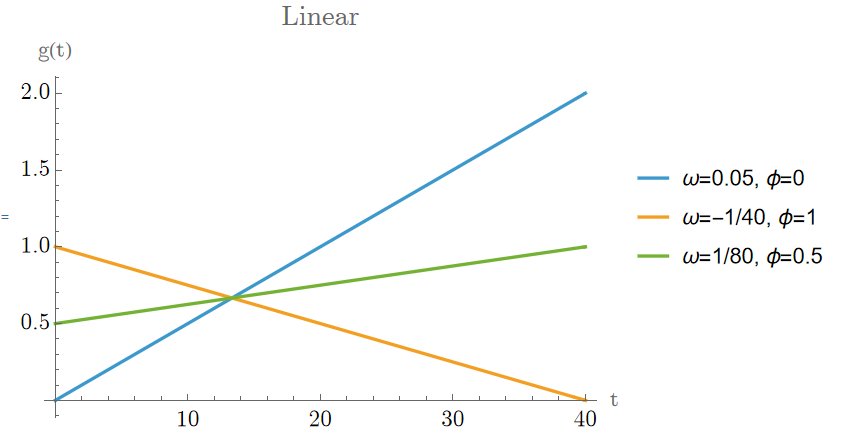
\includegraphics[width=0.9\linewidth]{images/linear.png}
    \caption{Exemplos de parâmetros para o acoplamento linear.}
\end{figure}


\section{Acoplamento Exponencial}

Agora, consideramos uma modulação do tipo \cite{Prants1995} 
\begin{equation}
    g(t)=g_0 \exp\left(\omega t+\phi\right).
\end{equation}

Intervalos de parâmetro interessantes:
\begin{itemize}
    \item Um aumento exponencial começando de um valor pequeno de acoplamento. 
    Exemplo:
    $\phi=\ln(10^{-3})$, $0<\omega<\frac{\ln(2)-\ln(10^{-3})}{40}$ (variação de um acoplamento pequeno  $g(0)=10^{-3}$ até um acoplamento $g(40)=2$, para $0<t<40$);
    \item Diminuição exponencial de um acoplamento que inicia em $1$.
    Exemplo:
    $\phi=0$, $\omega$ que simula um decaimento até $0$, $\frac{\ln(10^{-3})}{40}<\omega<0$ (para $0<t<40$);
    \item Aumento exponencial suave de um acoplamento que inicia em $1$.
    Exemplo: $\phi=0$, $0<\omega<\ln(2)/40$
    (variação de um acoplamento  $g(0)=1$ até um acoplamento $g(40)=2$, para $0<t<40$).
\end{itemize}

\begin{figure}
    \centering
    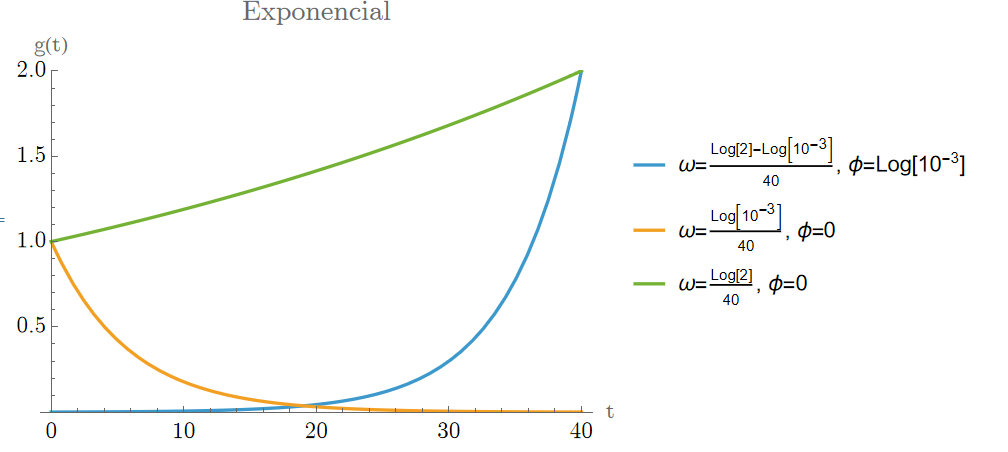
\includegraphics[width=0.9\linewidth]{images/exponencial_coupling.png}
    \caption{Exemplos de parâmetros para o acoplamento exponencial.}
\end{figure}

\section{Gaussian coupling}

Agora, consideramos uma modulação do tipo
\begin{equation}
    g(t)=g_0 \exp\left[\frac{\delta\left(  t-T\right)^2}{\zeta^2}\right],
\end{equation}
para cavidades Fabry-Perot. 

Nesse caso, temos o resultado de um pico nas quantidades consideradas, perto do pico da Gaussiana. 
O parâmetro $\delta$ controla o sinal somente (a concavidade da gaussiana), $T$ controla \emph{onde} o pico ocorre e $\zeta$ quão agudo é o fio.

Intervalos de parâmetro interessantes:
\begin{itemize}
    \item Considerando um pico exatamente no meio, para $0<t<40,\quad\delta=-1$, variamos a espessura do pico.
    Exemplo:
    $T=20$, $6<\zeta<10$.
    Não sei qual seria o mais próximo do real, mas é um intervalo grande.
    Para $\zeta$ ainda menores ($\zeta<1$), temos a Gaussiana se tornando uma $\delta$ de Dirac. 
    Não sei se isso é físico, mas talvez fosse interessante ver o que acontece;
    \item Também podemos variar a localização do pico, para $0<t<40,\quad\delta=-1$ e $\zeta=8$ (fixando a espessura). Também não sei o quão ``físico'' é isso.
    Exemplo:
    $15<T<25$. 
    \item Podemos obter uma gaussiana com concavidade oposta para $\delta=-1$ (fixando a localização e variando a espessura). Também não sei a praticidade experimental disso.
     Exemplo:
    $T=20$, $40<\zeta<45$ (esses parâmetros de $\zeta$ foram baseados em especulação do que resultaria em resultados legais, somente).
\end{itemize}

\begin{figure}
    \centering
    
\includegraphics[width=0.9\linewidth]{gaussian_coupling.png}
    \caption{Exemplos de parâmetros para o acoplamento gaussiano.}
\end{figure}

\printbibliography

\end{document}
